\documentclass[margin=5pt]{standalone}
\usepackage[utf8]{inputenc} 			
\usepackage[norsk]{babel}

\PassOptionsToPackage{gray}{xcolor}
\usepackage{tikz}
\usetikzlibrary{intersections,backgrounds}
\begin{document}

% List of colors

% Gradations
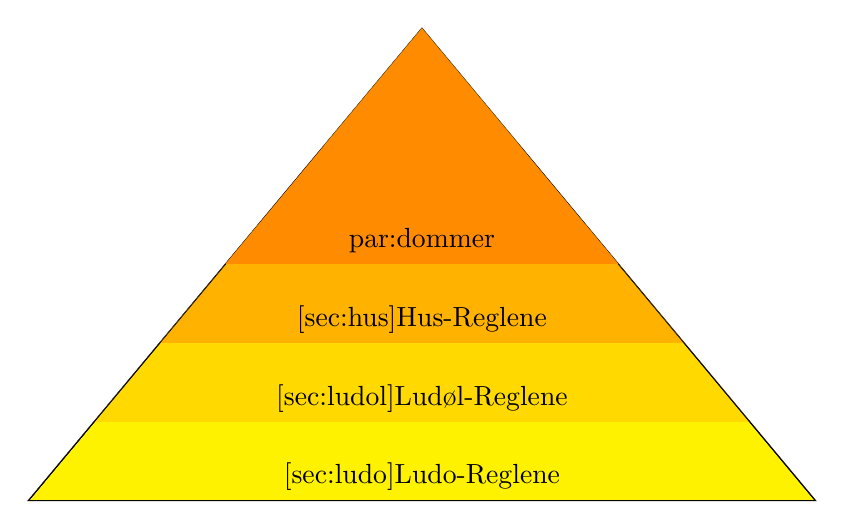
\begin{tikzpicture}[xshift=5cm]
\foreach \y/\A [count=\xi starting from 0, evaluate=\y as \nexty using (\y+1.5, evaluate=\xi as \grad using int(\xi*15)] in {0/\hyperref[sec:ludo]{Ludo-Reglene}, 1/\hyperref[sec:ludol]{Ludøl-Reglene}, 2/\hyperref[sec:hus]{Hus-Reglene},3/\Cref{par:dommer}} {%
    \begin{scope}[on background layer]
    \clip[preaction={draw}] (-5,0) -- (5,0) -- (0,6) -- cycle;
    \fill[red!\grad!yellow] (-5,\y) rectangle (5,\nexty);
    \fill[red!\grad!yellow] (-5,4.5) rectangle (5,7);
    \end{scope}
    \node at (0,\y+.3) {\A};
}
\end{tikzpicture}
\end{document}